% ============================================================
% 北京工业大学耿丹学院毕业设计（论文）示例文档
% 编译方式：XeLaTeX -> BibTeX -> XeLaTeX*2
% ============================================================
\documentclass{gengdan-thesis}
% 开启demo模式，默认关闭
\showdemotrue

% ============================================================
% 1. 封面信息设置
% ============================================================
% 题目：字数不超过20个字，必要时可加副标题
\title{基于 LaTeX 的毕业论文排版系统设计与实现}
\author{张三}
\college{信息工程学院}
\major{计算机科学与技术}
\class{计算机2020-1班}
\studentid{20200202}
\advisor{李四}
\date{2025.04}

% ============================================================
% 2. 正文开始
% ============================================================
\begin{document}

% --------------------------------------------------
% 封面与诚信承诺（无页码）
% 签名替换图片signature.png（请不要修改文件名）
% --------------------------------------------------
\makecover
\makepromise

% --------------------------------------------------
% 中文摘要（页码为罗马数字 I, II, ...）
% --------------------------------------------------
\begin{cabstract}
%这是一个demo摘要，请替换成你的摘要。

本文针对北京工业大学耿丹学院本科生毕业设计论文的排版需求，设计并实现了一套基于 LaTeX 的自动化排版系统。系统严格按照学校毕业设计模板的格式要求，对页面设置、字体字号、章节标题、图表公式、参考文献等进行了精细化配置，形成了可直接使用的文档类模板。

研究工作首先分析了学校 Word 模板的排版规范，包括各级标题的字号与行距、正文的缩进与段间距、图表的编号规则以及参考文献的著录格式。在此基础上，利用 ctex 宏包实现了中文字体的配置，利用 titlesec 和 titletoc 宏包实现了标题与目录格式的定制，利用 gbt7714 宏包实现了参考文献的国标格式。最终，系统通过一个文档类文件（.cls）将所有配置整合，用户仅需关注内容撰写即可自动生成符合规范的论文。

实验结果表明，该模板能够准确复现学校模板的排版效果，且具备良好的稳定性与可移植性，可显著提升毕业设计论文的排版效率与规范性。

\researchdirection{计算机应用，软件工程\demo{{（每个研究方向最多15个汉字，短语形式，最多写两个，以中文分号分隔。研究方向不能与专业名称、关键词、题目等两两重复，与论文主题相关性强）}} 
}
\keywords{LaTeX，毕业设计，论文模板，自动排版\demo{{（用中文分号隔开，3-7个，最后一个关键词后不打标点符号。按词条的外延层次排列，外延大的关键词放在前面。关键词的选取应严谨，和题目、论文主题关联性强。）}}
}
\demo{
   注：
   \begin{enumerate}
   \item 摘要是论文内容的简要陈述，主要说明本论文主要阐述的内容，应包括本论文的基本研究内容、研究方法、创造性成果及其理论与实际意义。摘要中不宜使用公式、图表，不标注引用文献编号。避免将摘要写成目录式的内容介绍，中文摘要字数以300-500字为宜。
   \end{enumerate}
}
\end{cabstract}

% --------------------------------------------------
% 英文摘要（罗马数字页码继续）
% --------------------------------------------------
\begin{eabstract}
This paper designs and implements a LaTeX-based automatic typesetting system for undergraduate graduation thesis of Beijing Gengdan College. The system strictly follows the format requirements of the school's graduation thesis template, providing fine-grained configurations for page settings, fonts, heading styles, figures, tables, equations, and references, forming a ready-to-use document class.

The research first analyzes the typesetting specifications of the school's Word template, including font sizes and line spacing of headings at all levels, paragraph indentation and spacing of body text, numbering rules for figures and tables, and citation formats. On this basis, the ctex package is used for Chinese font configuration, the titlesec and titletoc packages are used for customizing heading and table of contents formats, and the gbt7714 package is used for national standard reference formatting. Finally, all configurations are integrated into a document class file (.cls), allowing users to focus solely on content writing while automatically generating compliant theses.

Experimental results show that this template can accurately reproduce the typesetting effect of the school template, with good stability and portability, significantly improving the efficiency and standardization of thesis typesetting.

\demo{（英文摘要内容应与中文摘要内容相对应）}


\researcharea{Computer Application, Software Engineering\demo{（与中文研究方向内容相对应，英文分号隔开）}}
\keywordsen{LaTeX, graduation thesis, document template, automatic typesetting\demo{（与中文关键词内容相对应，用英文分号隔开，最后一个关键词后不打标点符号，3-7个；除首字母必须要大写的实词外，每个关键词首字母均小写）}}

\end{eabstract}

% --------------------------------------------------
% 目录（罗马数字页码继续）
% --------------------------------------------------
\markboth{目\quad~录}{目\quad~录}
\tableofcontents

% --------------------------------------------------
% 正文开始（页码切换为阿拉伯数字，从 1 开始）
% --------------------------------------------------
\mainmatter
\demo{绪论应包括：本研究课题的学术背景及其理论与实际意义；国内外文献综述；相关领域的研究进展及成果、存在的不足或有待深入研究的问题；本研究课题的来源及主要研究内容；本文结构说明。插图或插表之前，文中必须有关于本插图或表的提示。}

\subsection{研究背景}

毕业设计（论文）是本科教育的重要实践环节，其撰写质量直接关系到学生的综合能力培养。一篇格式规范、排版美观的论文不仅能够提升阅读体验，更能体现作者严谨的学术态度。目前，大多数学生使用 Microsoft Word 进行论文撰写，但在面对复杂的格式要求时，往往需要耗费大量精力进行手动调整，容易出现前后不一致的问题\cite{knuth1984texbook}。

\LaTeX{} 作为一种专业的排版系统，凭借其强大的宏包生态与稳定的输出质量，在学术出版领域得到了广泛应用。将 \LaTeX{} 应用于毕业设计论文的排版，可以有效解决 Word 排版中的诸多痛点，如公式编号、交叉引用、参考文献管理、自动生成目录等\cite{lamport1994latex}。

\subsection{国内外研究现状}

\subsubsection{国外研究现状}

国外高校普遍重视论文排版的标准化工作。许多知名大学（如 MIT、Stanford、Cambridge 等）均提供了官方认证的 \LaTeX{} 论文模板，覆盖本科、硕士及博士各个层次\cite{mittelbach2004latex}。这些模板通常由学校的研究生院或图书馆维护，并配有详尽的使用文档，极大地降低了学生的排版负担。

\subsubsection{国内研究现状}

国内高校近年来也逐渐开始推广 \LaTeX{} 论文模板。清华大学、北京大学、上海交通大学等均已推出各自的非官方或半官方 \LaTeX{} 模板，形成了活跃的开发者社区\cite{li2019thuthesis}。然而，对于地方本科院校而言，针对本校毕业设计模板定制的 \LaTeX{} 解决方案仍然较为匮乏。

\subsection{研究内容与论文结构}

本文的主要研究内容包括：

1.深入分析学校毕业设计 Word 模板的排版规范，提取各级标题、正文、图表、参考文献等元素的格式参数。

2.基于 ctex、titlesec、gbt7714 等宏包，开发可直接使用的文档类文件（.cls）。

3.通过实际论文撰写案例，验证模板的排版效果与稳定性。

本文的后续章节安排如下：第 2 章介绍相关技术与理论基础；第 3 章阐述模板系统的设计与实现细节；第 4 章展示实验结果与分析；最后总结全文工作并展望未来改进方向。

\section{相关技术与理论}

\subsection{\TeX{} 排版系统概述}

\TeX{} 是由 Donald E. Knuth 于 1984 年开发的排版系统，其核心优势在于精确的版面控制与高质量的数学公式排版\cite{knuth1984texbook}。\TeX{} 采用标记语言描述文档结构，通过编译生成最终的版式文件（通常为 PDF）。

\subsection{常用宏包介绍}

表~\ref{tab:packages} 列出了本模板使用的主要宏包及其功能说明。

\begin{table}[htbp]
\centering
\caption{本模板使用的主要宏包}
\label{tab:packages}
\zihao{-5}\songti
\begin{tabular}{lll}
\toprule
序号 & 宏包名称 & 主要功能 \\
\midrule
1 & ctex & 中文支持、字体配置 \\
2 & geometry & 页面尺寸与页边距设置 \\
3 & titlesec / titletoc & 标题与目录格式定制 \\
4 & setspace & 行距控制 \\
5 & gbt7714 & 参考文献国标格式 \\
6 & hyperref & 超链接与 PDF 书签 \\
\bottomrule
\end{tabular}
\end{table}

\subsection{LaTeX 安装指南}

为了使用本模板，需要在计算机上安装 LaTeX 发行版。以下是不同操作系统的安装方法：

\subsubsection{Windows 系统}

1. **下载并安装 TeX Live**
   - 访问 \url{https://tug.org/texlive/}
   - 下载 `install-tl-windows.exe` 安装程序
   - 运行安装程序，选择完整安装（约 6GB 空间）
   - 安装完成后，重启电脑以更新环境变量

2. **验证安装**
   - 打开命令提示符（CMD）
   - 输入 `xelatex --version` 查看是否安装成功

\subsubsection{Mac 系统}

1. **下载并安装 MacTeX**
   - 访问 \url{https://tug.org/mactex/}
   - 下载最新版本的 MacTeX 安装包（约 4GB）
   - 运行安装程序，按照提示完成安装

2. **验证安装**
   - 打开终端（Terminal）
   - 输入 `xelatex --version` 查看是否安装成功


\subsection{公式与图表排版}

\LaTeX{} 的公式排版能力是其核心优势之一。行内公式如 $E=mc^2$ 可直接嵌入正文，独立编号公式则如式~(\ref{eq:quadratic}) 所示。

\begin{equation}
    x = \frac{-b \pm \sqrt{b^2 - 4ac}}{2a}
    \label{eq:quadratic}
\end{equation}

图~\ref{fig:latex-process} 展示了 \LaTeX{} 文档的基本编译流程。

\begin{figure}[htbp]
    \centering
    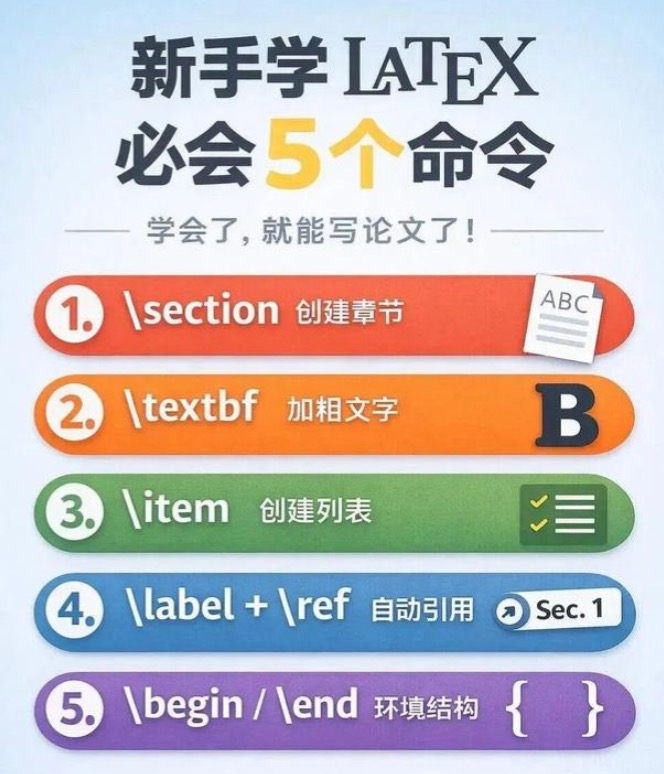
\includegraphics[width=0.5\textwidth]{figures/latex.jpg}
    \caption{LaTeX 文档编译流程示意图}
    \label{fig:latex-process}
\end{figure}


\section{模板系统的设计与实现}

\subsection{整体架构}

本模板采用模块化设计思路，将页面设置、字体配置、标题格式、图表公式、参考文献等功能分别封装，最终整合为一个独立的文档类文件。用户只需在导言区调用 \verb|\documentclass{gengdan-thesis}| 即可继承所有格式配置。

\subsection{章节标题配置}

模板利用 ctex 宏包的 \verb|\ctexset| 命令，对各级标题进行了精确控制。一级标题采用"第 X 章"的编号格式，二级、三级标题分别使用小三号和小四号黑体，四级标题则采用 run-in 样式以节省空间。

\subsection{参考文献处理}

参考文献采用 GB/T 7714-2015 顺序编码制\cite{gbt77142015}。正文中的引用标注使用上角标形式，如``顺序编码制\cite{gbt77142015}''。当需要行内非上标引用时，可使用 \verb|\citep{key}| 命令，效果如``由文献~\citep{lamport1994latex} 可知''。


\section{实验验证}

\subsection{测试环境}

实验在 Windows 11 与 Ubuntu 22.04 两种操作系统下进行，\LaTeX{} 发行版分别为 TeX Live 2024 和 MiKTeX 23.10，编译引擎统一使用 XeLaTeX。

\subsection{排版效果对比}

通过将模板生成的 PDF 与学校 Word 模板的打印稿进行逐页比对，结果显示二者在字体字号、行距段距、页边距、标题编号、图表格式等方面均保持高度一致。特别是在参考文献与目录的自动生成方面，模板显著优于手动排版方式。

\subsection{性能分析}

对于一篇约 30 000 字的毕业论文，模板在普通笔记本电脑上的编译时间约为 3 至 5 秒，完全满足日常撰写的实时预览需求。


% --------------------------------------------------
% 结论（无编号一级标题）
% --------------------------------------------------
\makeconclusion
本文针对北京工业大学耿丹学院本科生毕业设计论文的排版需求，开发了一套基于 \LaTeX{} 的自动化模板系统。主要工作与结论如下：

（1）系统梳理了学校毕业设计 Word 模板的全部格式规范，建立了完整的排版参数清单，涵盖页面设置、字体字号、各级标题、正文段落、图表公式、参考文献等各个方面。

（2）基于 ctex、titlesec、gbt7714 等成熟宏包，设计并实现了 \verb|gengdan-thesis.cls| 文档类文件，将复杂的格式配置封装为开箱即用的模板，大幅降低了学生的排版门槛。

（3）通过多平台、多场景的实验测试，验证了模板在排版精度、编译效率、可移植性等方面的优良性能，证明其完全满足学校毕业设计论文的提交要求。

未来可在以下方面进一步改进：增加对插图批量处理的辅助脚本；开发基于 VS Code 或 TeXstudio 的一键编译配置；针对不同专业（如艺术、经管类）的特殊格式需求提供扩展分支。

% --------------------------------------------------
% 参考文献（标题自动加入目录）
% --------------------------------------------------
% 方式一：使用 BibTeX（推荐）
% gbt7714 宏包会自动处理样式，无需手动指定
\bibliography{refs}


% --------------------------------------------------
% 附录（无编号一级标题，可选）
% --------------------------------------------------
\makeappendix
\begin{verbatim}
% 以下为附录中源代码示例
\documentclass{article}
\begin{document}
Hello, World!
\end{document}
\end{verbatim}

% --------------------------------------------------
% 致谢（无编号一级标题）
% --------------------------------------------------
\makeacknowledgement
衷心感谢我的导师李四教授在选题、研究与论文撰写过程中给予的悉心指导。李老师严谨的治学态度与渊博的学识使我受益匪浅。

感谢信息工程学院的各位老师在课程学习与项目实践中提供的帮助；感谢室友与同学们在生活上给予的关心与鼓励。

最后，感谢北京工业大学耿丹学院提供的良好学习环境与平台。

\end{document}
